\newcommand{\pluginName}{Point Function 2D}
\newcommand{\pluginVersion}{1.0.2}

\input{../../../DocumentationTemplate/TemplateL3}

\begin{document}
\PluginTitle{\pluginName}{\pluginVersion}

\section{Introduction}
The \emph{Point Function 2D} plug-in allows you to define a bi-dimensional function defined by given control points. Function values are, then, generated by interpolation or extrapolation.

The plug-in implements 3 types of interpolation:
\begin{itemize}
\item Bi-linear interpolation
\item zero order interpolation
\item left zero order interpolation
\end{itemize}

The function values outside the domain specified by control points is given by constant extrapolation (the value at the nearest available data point is used).

\section{How to use the plug-in}
In the Fairmat user interface, when adding a new parameter \& functions, you will find the additional option \emph{2D Function defined by value interpolation} under functions.
You will then be shown a window similar to the one used to define the 1D version of this plug-in, except that you will be given the freedom to define as many columns and as many rows as you wish (See also Figure~\ref{fig.PFunction2DGUI}).

\begin{figure}[ht]
\begin{center}
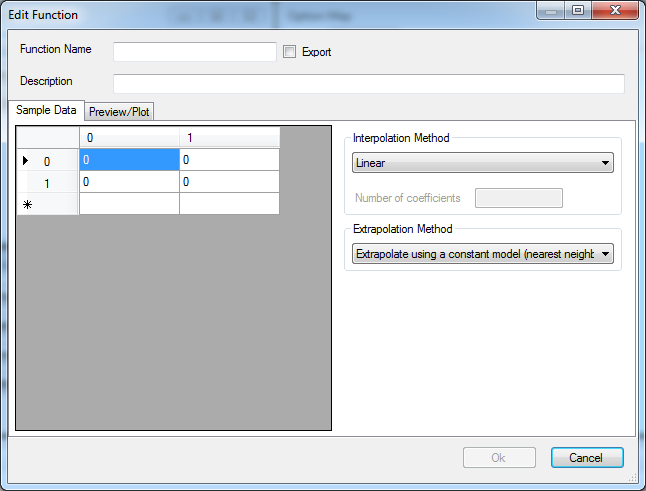
\includegraphics[width=0.48\textwidth]{./images/PFunction2DEdit.png}
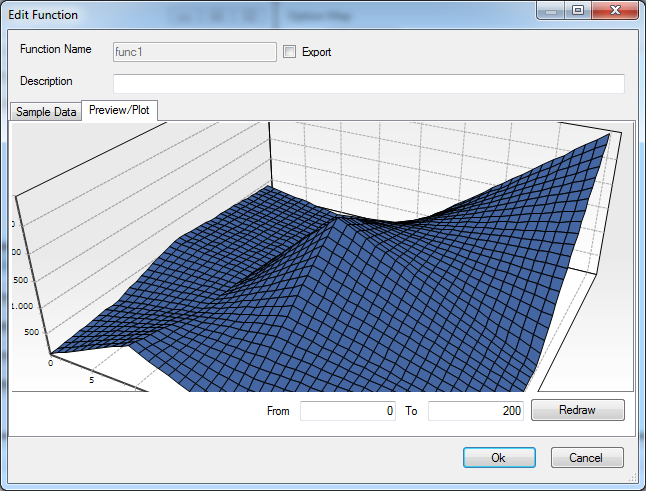
\includegraphics[width=0.48\textwidth]{./images/PFunction2DPreview.png}
\caption{Point Function 2D GUI: input parameters editor and preview.}
\label{fig.PFunction2DGUI}
\end{center}
\end{figure}

In order to give values to coordinates, you can double click on the row/column header, which will show you a window allowing you to change them (See also Figure~\ref{fig.PFunction2DColumnEdit}). Additionally you can add/remove columns by right clicking on the column headers and by selecting one of the contextual options, allowing you to remove or insert them before or after the one you are working on. The same identical procedure can be done with rows.

As for filling in the data points, you just need to fill in the single cells which will appear when creating rows or columns.

\begin{figure}[ht]
\begin{center}
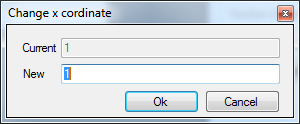
\includegraphics[width=0.48\textwidth]{./images/PFunction2DColumnEdit.png}
\caption{Editing rows and colunns cordinate values.}
\label{fig.PFunction2DColumnEdit}
\end{center}
\end{figure}

You have the freedom to use any formula for coordinates and point values, but remember that during evaluation, rows and columns coordinates must be ordered in ascending order (they must increase while going from left to right and from top to bottom) or you'll get an error during evaluation.

Finally, on the right of the form, you can choose the interpolation and extrapolation methods you want to apply to the function evaluation.
\section{Interpolation implementation}
These formulas are used to implement the interpolations.
\subsection{Bi-linear interpolation}
$f(x, y) = \frac{f(x_1, y_1)}{(x_2 - x_1)(y_2 - y_1)}(x_2 - x)(y_2 - y) + \frac{f(x_2, y_1)}{(x_2 - x_1)(y_2 - y_1)}(x - x_1)(y_2 - y) + \frac{f(x_1, y_2)}{(x_2 - x_1)(y_2 - y_1)}(x_2 - x)(y - y_1) + \frac{f(x_2, y_2)}{(x_2 - x_1)(y_2 - y_1)}(x - x_1)(y - y_1)$

where:
\begin{itemize}
\item $x_1$ is the coordinate before $x$
\item $x_2$ is the coordinate after $x$
\item $y_1$ is the coordinate before $y$
\item $y_2$ is the coordinate after $y$
\end{itemize}
\subsection{Linear interpolation}
This is used when the bi-linear interpolation is not applicable (e.g. The points have the same x/y axis).

$f(x) = y_0 + \frac{(x - x_0)y_1 - (x - x_0)y_0}{x_1 - x_0}$

where:
\begin{itemize}
\item $x_0$ is the coordinate before $x$
\item $x_1$ is the coordinate after $x$
\item $y_0$ is the value of the function at $x_0$
\item $y_1$ is the value of the function at $x_1$
\end{itemize}
\end{document}
